\documentclass[../thesis.tex]{subfiles}
\begin{document}
\chapter{Introduction}\label{chap:intro}
\lipsum[1]

\section{example of equation}
\begin{gather}
    y = g(z) \quad \forall z \in \R
\end{gather}
\subsection{example of multiline equations}
this is a \verb|gather| environment
\begin{gather}
    y = f(x)\\
    z = g(\omega) + \Gamma(\tau)
\end{gather}
this is an \verb|align| environment
\begin{align}
    y = f(x) \\
    z = g(\omega) + \Gamma(\tau)
\end{align}
this is an \verb|align| environment with text aligned to the left
\begin{align}
    & y = f(x) \\
    & z = g(\omega) + \Gamma(\tau)
\end{align}
this is a \verb|dcases| environment
\begin{gather}
    \delta(x) = 
    \begin{dcases}
        +\infty, &\text{ if } x = 0\\
        0, &\text{ if } x \neq 0
    \end{dcases}
\end{gather}
A detailed description of multiline math environments is given in \href{https://github.com/marco-coraggio/scientist-s-matchbox}{\textcolor{blue}{Marco Coraggio's scientist's matchbox}} (note here an example of how to create a clickable link to a website and how to \textcolor{red}{colour text})


\section{example of figure inclusion}
\begin{figure}
    \centering
    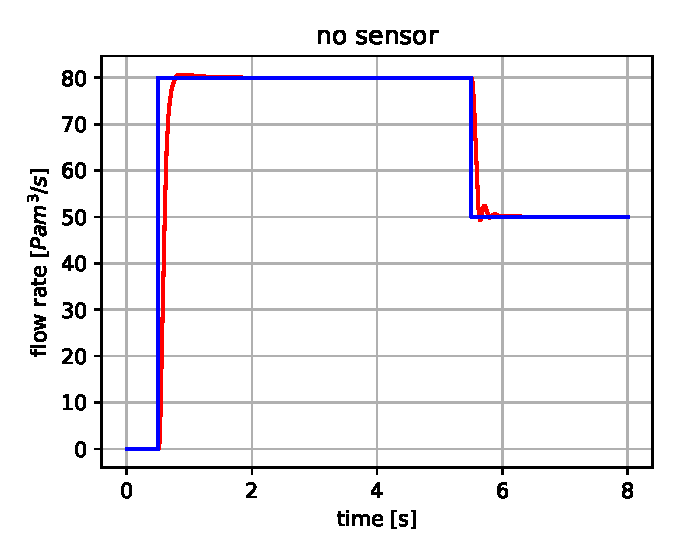
\includegraphics[width=0.75\textwidth]{control_no_sensor}
    \caption{controlled valve with no simulated sensor}
    \label{fig:cns}
\end{figure}

\subsection{multiple figures side by side}
we have two main options: 
\begin{figure}
    \centering
    \begin{subfigure}[b]{0.49\textwidth}
        \centering
        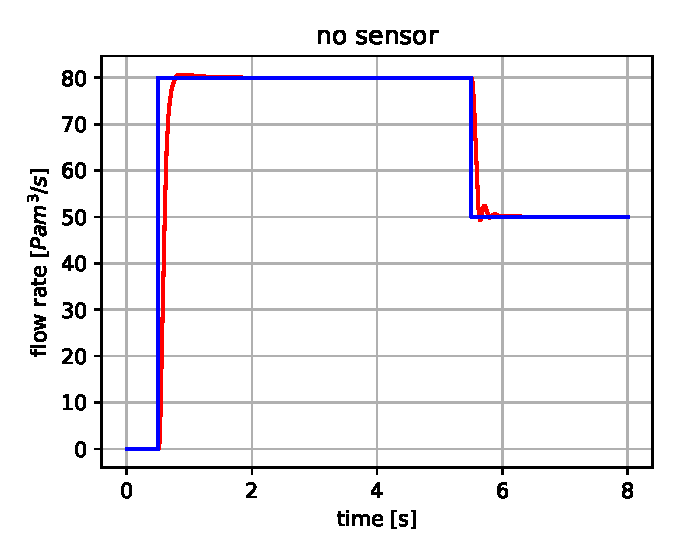
\includegraphics[width=\textwidth]{control_no_sensor}
        \caption{subfigure 1}\label{fig:subfig1}
    \end{subfigure}
    \begin{subfigure}[b]{0.49\textwidth}
        \centering
        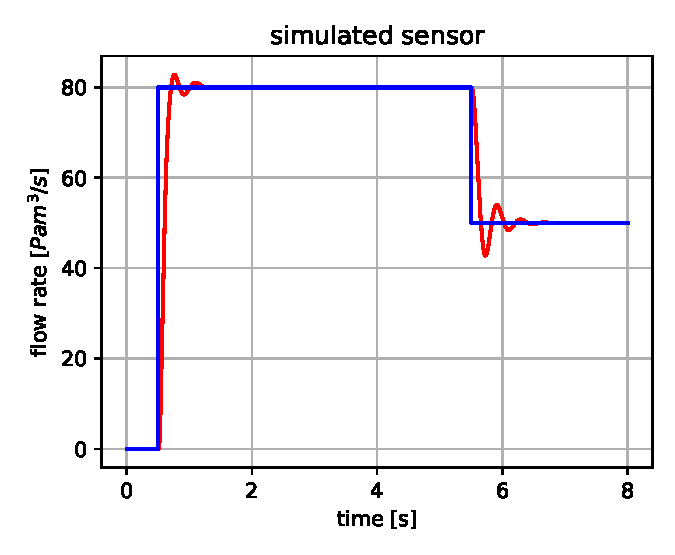
\includegraphics[width=\textwidth]{control_simulated_sensor}
        \caption{subfigure 2}\label{fig:subfig2}
    \end{subfigure}
    \caption{subfigure environment gets subcaptions}
\end{figure}


\begin{figure}
\centering
\begin{minipage}{.5\textwidth}
  \centering
  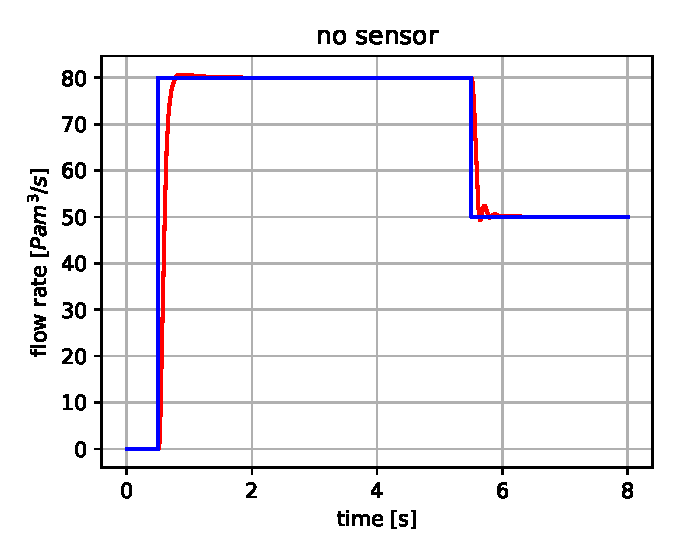
\includegraphics[width=.95\linewidth]{control_no_sensor}
  \captionof{figure}{minipage 1}
  \label{fig:mini1}
\end{minipage}%
\begin{minipage}{.5\textwidth}
  \centering
  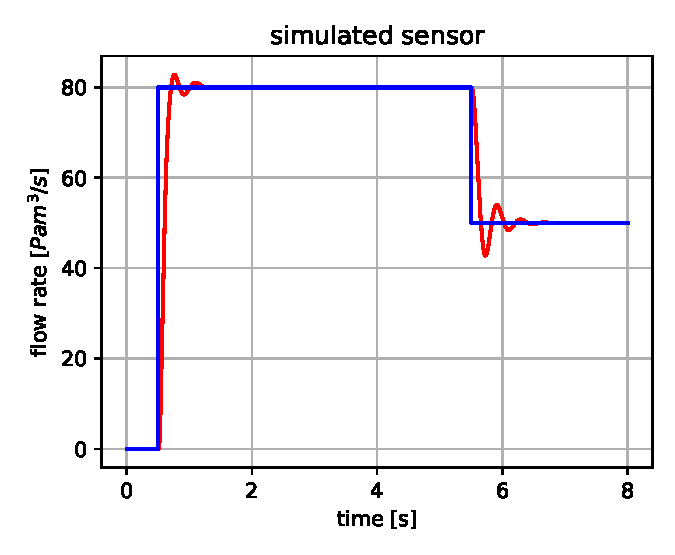
\includegraphics[width=.95\linewidth]{control_simulated_sensor}
  \captionof{figure}{minipage 2}
  \label{fig:mini2}
\end{minipage}
\caption{each figure gets its own caption in minipages, so if you add one for all the images numbering gets messed up!}
\end{figure}


\section{tables}
To make tables you can go to \href{https://www.tablesgenerator.com/}{a table generator online} to avoid writing out all the boring syntax. 
\begin{table}[h]
\centering
\begin{tabular}{|l|l|l|l|l|}
\hline
a & b & c & d & e \\ \hline
f & g & h & i & j \\ \hline
k & l & m & n & o \\ \hline
p & q & r & s & t \\ \hline
\end{tabular}
\caption{the firs 20 letters of the alphabet}
\label{tab:table}
\end{table}

\section{referencing document elements} \label{sec:ref}
here a short and definitely incomplete list of document elements that can be referenced. Necessary condition for something to be referenced is that it be assigned a \verb|\label|
\begin{itemize}
    \item Chapters: you can click on the number and be sent to chapter \ref{chap:intro}  
    \item Sections: you can click on the number and be sent to section \ref{sec:ref}
    \item Images: you can click on the number and be sent to section \ref{fig:mini1}
    \item tables: you can click on the number and be sent to section \ref{tab:table}
\end{itemize}
\subsection{citations}
in order to include citations a \verb|.bib| file is used (here found in \verb|./resources/bibliography.bib|). Some examples are included here, as \cite{dumb} to learn why being stupid is good for research, or \cite{drinking} to use as an excuse to show up to work drunk, or \cite{integration} to see a biologist reinventing Riemann integration, or finally \cite{booba} just to be aware people publish papers about anime tiddies. As you can see citations are ordered alphabetically rather than in the order they appear in the text. Also, they're hyperlinked to the bibliography! (We love the \verb|hyperref| package)


\end{document}
